\documentclass[9pt,conference]{IEEEtran}
\usepackage{cite}
\usepackage{amsmath,amssymb,amsfonts}
\usepackage{multirow}
\usepackage{array}
\usepackage{graphicx}
\usepackage{textcomp}
\usepackage{xcolor}
\usepackage{algorithm}
\usepackage[noend]{algpseudocode}
\usepackage{hhline}
\usepackage{amsmath}
\usepackage{mathrsfs}
\usepackage{hyperref} % For clickable references
\graphicspath{{Figures/}}
\def\BibTeX{{\rm B\kern-.05em{\sc i\kern-.025em b}\kern-.08em
    T\kern-.1667em\lower.7ex\hbox{E}\kern-.125emX}}
\begin{document}

\title{Design and Analysis of Voltage Multiplier Circuits}
\author{\IEEEauthorblockN{B23500, B23495, B23504 and B23303}
\IEEEauthorblockA{\textit{EE - 211P} \\
Lab Report 1}
}
\maketitle

\begin{aim}
AIM: To design and analyze voltage multiplier circuits using clamper circuits and peak detectors, and to verify their functionality through practical implementation.
\end{aim}

\begin{abstract}
This experiment demonstrates the working of voltage multipliers using clamper circuits and peak detectors. The objective is to determine how a clamper modifies the DC level of an AC signal without distorting its shape and how a peak detector accumulates the peak voltage of a waveform. By cascading these circuits, a voltage multiplier is built to boost DC output. Practical results are compared with theoretical predictions to analyze the effectiveness of these designs. The study highlights the importance of these circuits in signal processing and power electronics, where efficient voltage control is critical.
\end{abstract}

\begin{IEEEkeywords}
Voltage Multiplier, Clamper Circuit, Peak Detector, Voltage Doubler, Xcircuit.
\end{IEEEkeywords}

\section{Introduction}
Voltage multipliers are essential in applications requiring higher DC voltages than those available directly from power sources. This experiment explores the design and functionality of voltage multipliers using clamper circuits and peak detectors. The circuits were constructed on a breadboard and analyzed using a Digital Storage Oscilloscope (DSO) and a function generator. The study focuses on the theoretical and practical aspects of these circuits, including their implementation.

\section{Working Principle}
Voltage multipliers operate by incrementally increasing DC voltage using a series of peak detection and clamping circuits. These circuits utilize diodes to regulate current flow and capacitors to store energy, enabling step-by-step voltage increases.

\subsection{Clamper Circuit – Voltage Level Adjustment}
A clamper circuit adjusts the DC level of a signal without altering its shape. It uses a capacitor to store charge and a diode to control the voltage shift. The capacitor charges near the negative peak of the signal, and the stored charge pumps the waveform to a new DC level as the signal rises. This technique is widely used in communication systems for DC restoration and waveform conditioning.

\subsection{Peak Detector – Recording Maximum Voltage}
A peak detector stores the highest voltage reached by an AC signal. It consists of a diode for unidirectional current flow and a capacitor for storing the peak value. The capacitor retains the peak voltage until it is recharged. Peak detectors are commonly used in power monitoring, signal measurement, and modulation circuits.

\subsection{Voltage Multiplier – Boosting DC Output}
By cascading clamper and peak detector circuits, a voltage multiplier is created. Successive stages add a controlled voltage boost:
- A voltage doubler produces nearly double the input voltage.
- Additional stages can be used for higher voltage gains.
This method is employed in power supply circuits, high-voltage generators, and RF communication systems.

\section{Practical Implementation and Results}
The experiment tested the performance of voltage doubler and higher multiplication circuits. The circuits were implemented using diodes and capacitors based on the principles of clamper and peak detector circuits. 

\begin{figure}[H]
\centering
\includegraphics[width=0.4\textwidth]{peak_det_ckt_pos.eps}
\caption{\label{fig:peak_detector}Peak Detector Circuit.}
\end{figure}

\subsection{Clamper and Peak Detector Results}
- Clamper Circuit: As seen in the transient response (Figure \ref{fig:transient_clamper}), the waveform is clamped by approximately 2.45 V. This is calculated as \(3 \, \text{V} - 0.7 \, \text{V}\), where \(0.7 \, \text{V}\) is the diode's threshold voltage. The clamper successfully shifts the DC level of the input signal without distorting its shape.\\
- Peak Detector: The peak detector (Figure \ref{fig:peak_detector}) accurately captures the peak voltage of the input signal. However, a slight difference is observed between the theoretical and measured peak values due to diode forward voltage drops and capacitor inefficiencies.

\begin{figure}[H]
\centering
\includegraphics[width=0.4\textwidth]{clamper_ckt_pos.eps}
\caption{\label{fig:clamper}Clamper Circuit.}
\end{figure}

\begin{figure}[H]
\centering
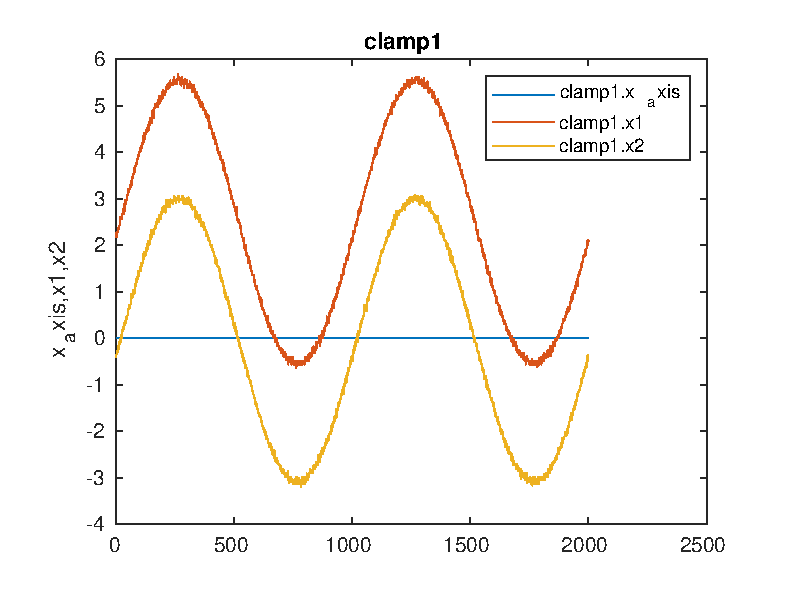
\includegraphics[width=0.5\textwidth]{clamp.eps}
\caption{\label{fig:transient_clamper}Transient Response of Clamper Circuit.}
\end{figure}

\subsection{Voltage Doubler Implementation}
\begin{figure}[H]
\centering
\includegraphics[width=0.4\textwidth]{Doubler_ckt.eps}
\caption{\label{fig:voltage_doubler}Voltage Doubler Circuit.}
\end{figure}

- A voltage doubler circuit (Figure \ref{fig:voltage_doubler}) was constructed using two diodes and two capacitors in a charge-pump configuration.
- A 6 peak-to-peak (Vpp) AC input was applied.
- The output voltage was approximately 5V DC, close to theoretical expectations.
- Minor voltage drops occurred due to diode forward voltage drops, but the circuit performed as expected.

\begin{figure}[H]
\centering
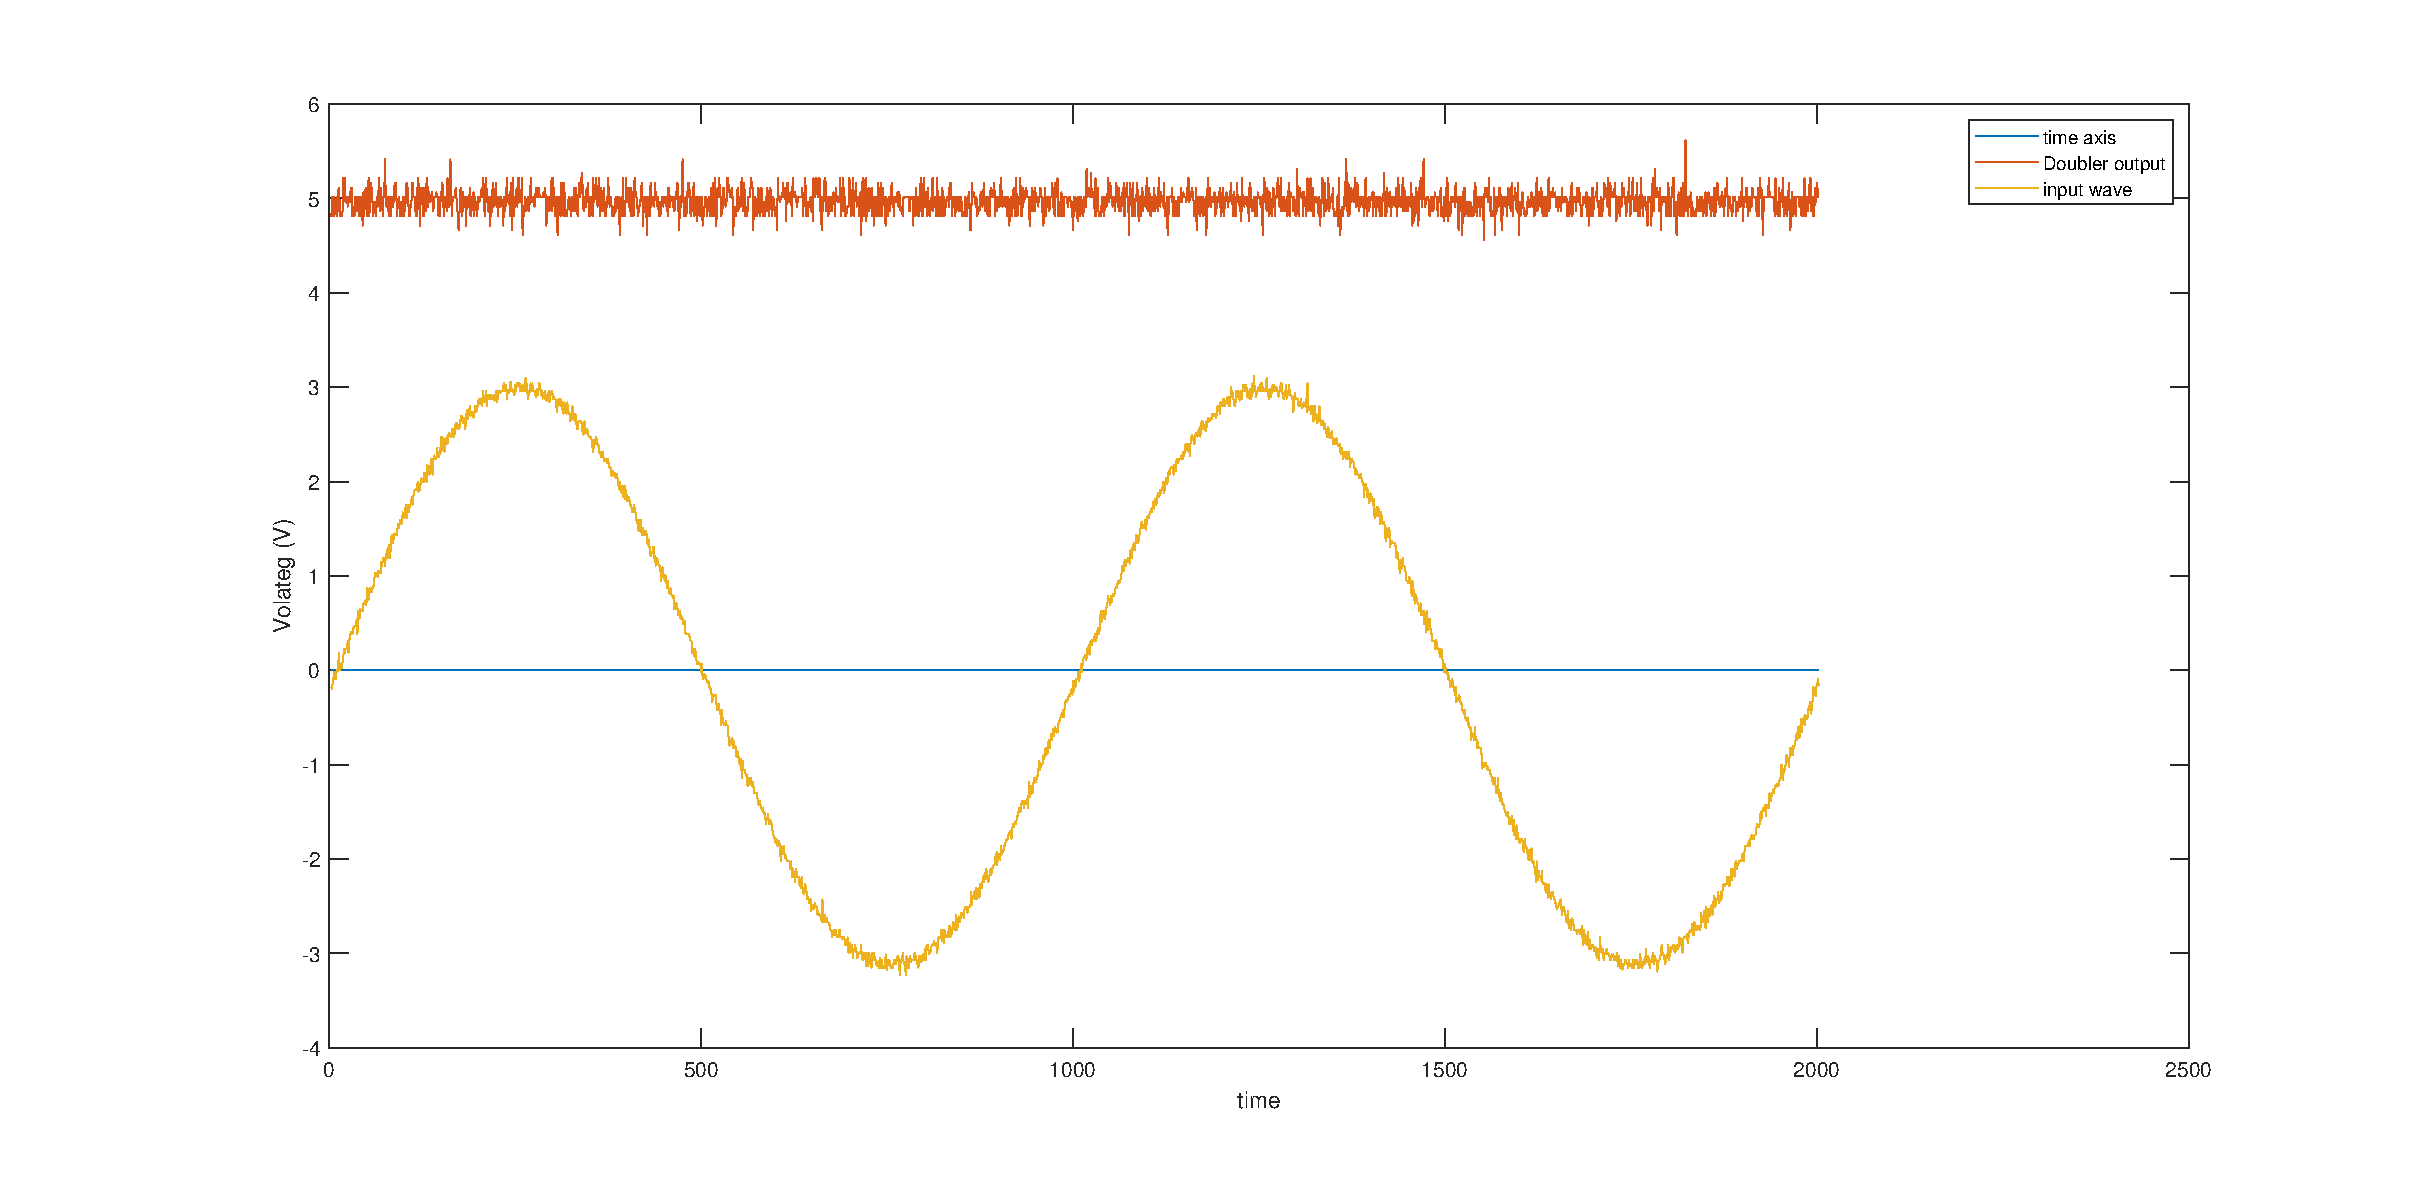
\includegraphics[width=0.5\textwidth]{doubler.eps}
\caption{\label{fig:transient_doubler}Transient Response of Voltage Doubler Circuit.}
\end{figure}

\subsection{Higher Voltage Multiplier Implementation}
\begin{figure}[H]
\centering
\includegraphics[width=0.5\textwidth]{penta_multiplier.eps}
\caption{\label{fig:voltage_penta}Voltage Penta Multiplier Circuit.}
\end{figure}

- A five-stage voltage multiplier (Figure \ref{fig:voltage_penta}) was implemented.
- An unidentified error resulted in an incorrect output waveform.
- The circuit was rechecked for errors, but none were found.
- Despite careful wiring to avoid parasitic capacitance, the circuit did not function as expected.

\subsection{Results and Observations}
- The voltage doubler successfully doubled the input, producing a 5V DC output from a 3Vpp AC input.
- The five-stage voltage multiplier did not function correctly due to an unidentified issue.
- Output voltage losses were observed due to diode forward voltage drops and capacitor inefficiencies.
- The experiment demonstrated that cascading diode-capacitor circuits allows effective voltage multiplication with minimal complexity.

\begin{figure}[H]
\centering
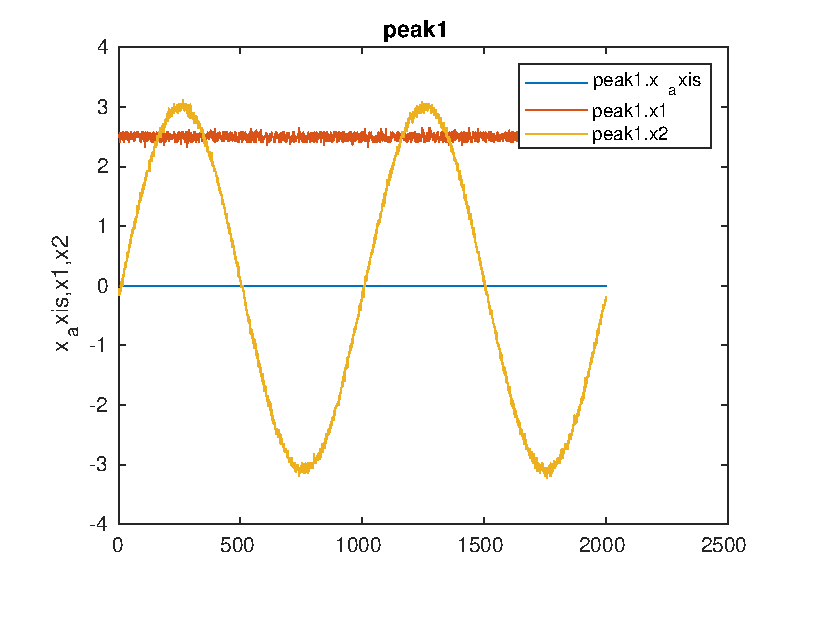
\includegraphics[width=0.5\textwidth]{peak.eps}
\caption{\label{fig:transient_peak}Transient Response of Peak Detector Circuit.}
\end{figure}

\begin{figure}[H]
\centering
\includegraphics[width=0.5\textwidth]{penta_board.png}
\caption{\label{fig:physical}Physical Implementation of Voltage Penta Multiplier on Breadboard.}
\end{figure}

\section{Discussion}
Voltage multipliers are crucial in applications requiring higher DC voltages. The experiment demonstrated the effectiveness of clamper circuits and peak detectors in achieving voltage multiplication. While the voltage doubler performed as expected, the five-stage multiplier encountered issues, highlighting practical limitations such as diode drops and parasitic capacitance. These findings underscore the importance of careful design and implementation in power electronics.

\section{Conclusion}
This experiment successfully demonstrated the working of clamper circuits, peak detectors, and voltage multipliers. The clamper circuit shifted the DC level of the signal, the peak detector stored the maximum voltage, and the voltage doubler effectively doubled the input voltage. Although the five-stage voltage multiplier did not function as expected, the experiment provided valuable insights into practical challenges. The study confirmed the significance of diode-capacitor voltage multipliers in power electronics and signal processing applications.

\begin{thebibliography}{00}
\bibitem{1}
Razavi, B. (2000). \textit{Design of Analog CMOS Integrated Circuits}. McGraw-Hill. \url{https://www.mheducation.com/}

\bibitem{2}
Sedra, A. S., & Smith, K. C. (2016). \textit{Microelectronic Circuits} (7th ed.). Oxford University Press. \url{https://global.oup.com/}

\bibitem{3}
XCircuit Documentation – Available at: \url{http://opencircuitdesign.com/xcircuit/}
\end{thebibliography}
\end{document}